\textbf{Introduction}\\
Au cours de ce dernier chapitre nous allons entamer le troisième sprint. 
\section{Sprint Planning Meeting}
\subsection{Objectif de Sprint}
Au cours de ce troisième sprint, nous allons développer les fonctionnalités reliées aux EPIC:
\begin{itemize}
	\item Gestion d'inscription. 
	\item Interaction sur le site.
\end{itemize}
Le développement du sprint va passer par les étapes suivantes: Analyse, conception et réalisation.
\subsection{Backlog du troisième Sprint}
L'élaboration du sprint backlog du troisième sprint à partir du Backlog product est présentée dans le tableau suivant:
\newpage
\begin{table}[!h]
	\centering % used for centering table
	\begin{tabular}{|c|p{6cm}|p{6cm}|c|}
		\hline
		\textbf{Id}&\textbf{User Story} & \centering{\textbf{Sprint Backlog Item}} & \textbf{Effort}\tabularnewline
		\hline
		\multirow{3}{*}{US7}&\multirow{3}{6cm}{ En tant qu'utilisateur, je veux m'inscrire pour pouvoir participer à une formation }&Développer un plugin pour créer un nouveau type de contenu&5\\
		\cline{3-4}
		&&Activer le plugin d'inscription &1\\
	
		&&  &\\
		\hline
		\multirow{3}{*}{US8}&\multirow{3}{6cm}{En tant qu'administrateur ou apprenant, je veux m'authentifier}&Développer l'API de connexion&3\\
		\cline{3-4}
		&&Réaliser l'interface de connexion &3\\
		\cline{3-4}
		&&Consommer l'API de connexion &3\\
		\hline
		\multirow{3}{*}{US9}&\multirow{3}{6cm}{En tant qu'administrateur, je peux confirmer une inscription}&Créer un nouveau type de contenu personnalisé&3\\
		\cline{3-4}
		&&Utiliser le type créé pour faire l'ajout d'un apprenant &2\\
		\hline
		\multirow{3}{*}{US10}&\multirow{3}{6cm}{En tant qu'administrateur ou apprenant, je peux donner une note concernant une formation}&Développer l'API pour noter une fromation&3\\
		\cline{3-4}
		&&Réaliser l'élément de l'interface qui permet à un apprenant de noter une formation &5\\
			\cline{3-4}
		&&Consommer l'API&3\\
		\hline
		\multirow{3}{*}{US11}&\multirow{3}{6cm}{En tant qu'administrateur ou apprenant, je peux modifier une note concernant une formation}&Développer l'API pour noter une formation&3\\
		\cline{3-4}
		&&Réaliser l'élément de l'interface qui permet à un apprenant de noter une formation &3\\
		\cline{3-4}
		&&Consommer l'API&3\\
		\hline
		\multirow{3}{*}{US12}&\multirow{3}{6cm}{En tant qu'administrateur ou apprenant, je peux supprimer une note concernant une formation}&Développer l'API pour supprimer une note&5\\
		\cline{3-4}
		&&Réaliser l'élément de l'interface qui permet à un apprenant de supprimer une note &3\\
		\cline{3-4}
		&&Consommer l'API&3\\
		\hline
		
		
		
		
		
	\end{tabular}
	\caption{Tableau : Backlog Sprint 3}
\end{table} 
\section{Analyse}
\subsection{Diagramme des cas d'utilisation}
\begin{itemize}
	\item Diagramme de cas d'utilisation globale du sprint 3
	\newpage
	\begin{figure}[!h]
		\centering
		{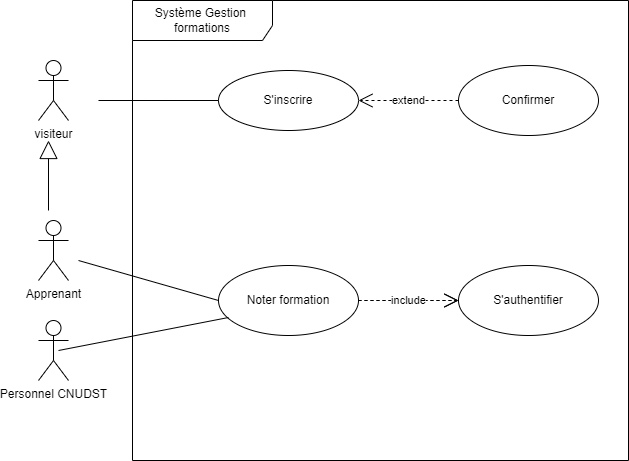
\includegraphics[width=0.95\textwidth]{D) IMAGES/digcha5.png}}
		\caption{Interface :Diagramme du cas d'utilisation globale-sprint 3 }
		\label{Org}
	\end{figure}

\item Détails du cas d'utilisation globale<<Noter formation>>

\begin{figure}[!h]
	\centering
	{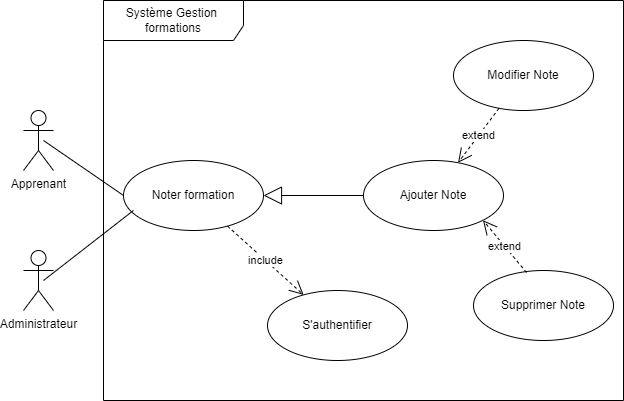
\includegraphics[width=0.95\textwidth]{D) IMAGES/detchap5.png}}
	\caption{Détails du cas d'utilisation "Noter formation" }
	\label{Org}
\end{figure}
\end{itemize}
\section{Description textuelle des cas d'utilisation}
\subsection{Cas d'utilisation "S'inscrire"}
Description textuelle du cas d'utilisation "S'inscrire"\\
\textbf{Titre :} Cas d'utilisation: s'inscrire\\
\textbf{But:} Détailler les étapes permettant à un visiteur de s'inscrire à une formation.\\
\textbf{Acteur Principal:} visiteur\\
\textbf{Date de création:} 27/07/2022\\
\textbf{Date de mise à jour:} 09/08/2022\\
\textbf{Responsable:} Olfa CHAOUECH\\
\textbf{Version:} 1.0\\
\textbf{Description des scénarii:}\\
Le cas d'utilisation commence quand un visiteur choisit une formation et veut s'inscrire.

\textbf{Pré condition:}\\
Le visiteur n'a pas encore choisi une formation.\\
\textbf{Scénario nominal:}
\begin{enumerate}
	\item le visiteur choisit une formation.
	\item Le visiteur clique sur la formation choisie. 
	\item Le système affiche la page détails formation qui présente un lien de redirection vers la page d'inscription.
	\item Le visiteur clique sur le bouton s'inscrire.
	\item Le système redirige le visiteur vers le formulaire d'inscription.
	\item Le visiteur remplit le formulaire avec les champs requis.
	\item Le visiteur clique sur le bouton envoyer.
	\item Le système vérifie les données saisies en fonction des conditions de validation.
	\item Le système insère les données du visiteur dans la base.
	\item L'administrateur confirme l'inscription.\\
	\textbf{Scénario Alternatif A:}\\
	A1 : Un ou plusieurs champs requis du formulaire sont non remplis.
	$\rightarrow$ L'enchaînement A1 démarre au point 6 de scénario nominal.\\
	7- Le système reste sur le formulaire d'inscription et indique qu'il y'a un ou plusieurs champs manquants qu'il faut compléter.\\
	$\rightarrow$ Le scénario reprend au point 5.\\
	A2 : Données reconnues par le système comme déjà enregistrée dans la base\\
	$\rightarrow$ L'enchaînement A2 démarre au point 8 de scénario nominal.\\
	8- Le système affiche un message indiquant que l'utilisateur existe dans la base.\\
	9- Le système réaffiche le formulaire d'inscription pour que le visiteur ressaisit ses données.\\
	$\rightarrow$ Le scénario reprend au point 5.
	
	\textbf{Scénario d'exception E:}\\
	E1 : L'utilisateur est déjà inscrit.\\
		$\rightarrow$ L'enchaînement E1 démarre au point 9 du scénario nominal.\\
	9- Le système réaffiche le formulaire d'inscription pour que l'utilisateur ressaisit ses données.\\
	10- L'utilisateur saisi des nouvelles données.\\ 
	11- L'utilisateur quitte la page.\\
	$\rightarrow$ L'enchaînement E1 démarre au point 3 du scénario nominal.\\
	

\end{enumerate}
\textbf{Post-condition:}\\
L'inscription se fait avec succès.





\subsection{Cas d'utilisation "Noter Formation"}
Description textuelle du cas d'utilisation "Noter Formation"
\textbf{Titre :} Cas d'utilisation: Noter Formation\\
\textbf{But:} Détailler les étapes permettant à un visiteur de noter une formation.\\
\textbf{Acteur Principal:}apprenant\\
\textbf{Date de création:} 25/08/2022\\
\textbf{Date de mise à jour:} 26/08/2022\\
\textbf{Responsable:} Olfa CHAOUECH\\
\textbf{Version:} 1.0\\
\textbf{Description des scénarii:}\\
Le cas d'utilisation commence quand un apprenant s'authentifier et clique sur le bouton My Notes.

\textbf{Pré condition:}\\
Le visiteur n'a pas encore inscrit.\\
\textbf{Scénario nominal:}
\begin{enumerate}
	\item L'apprenant s'authentifie.
	\item L'apprenant clique sur le bouton "My Notes" de la barre de menu. 
	\item Le système affiche la page "My Notes".
	\item L'apprenant ajoute une note sur une formation.
	\item L'apprenant valide l'ajout en cliquant sur le bouton Create Note.
	\item Le système affiche la note ajoutée.
	\item Quand l'administrateur ou l'apprenant choisit  de modifier la note ajoutée, il clique sur "Edit" .
	\item Le système affiche un formulaire pour modifier la note.
	\item L'administrateur ou l'apprenant saisit la modification désirée.
	\item L'administrateur ou l'apprenant clique sur le bouton "save".
	\item Le système affiche la note modifiée.
	\item Quand l'administrateur ou l'apprenant choisit de supprimer une note, il clique sur "delete".
 
	
	\textbf{Scénario Alternatif A:}\\
	A1 : L'utilisateur est sur la page et veut ajouter une autre note.
	$\rightarrow$ L'enchaînement A1 démarre au point 4 de scénario nominal.\\
	5- L'apprenant valide l'ajout en cliquant sur le bouton "Create Note" \\
	6- Le système affiche la note ajoutée.\\
	$\rightarrow$ L'enchaînement A1 démarre au point 7 de scénario nominal.\\
	\textbf{Scénario d'exception E:}
	E1 : L'utilisateur dépasse le nombre maximal de notes ajoutées.\\
	$\rightarrow$ L'enchaînement E1 démarre au point 11 du scénario nominal.\\ 
	12- L'utilisateur saisit une nouvelle donnée.\\ 
	13- L'utilisateur clique sur le bouton save.\\
	14- La note est ajoutée et l'utilisateur quitte la page.
	$\rightarrow$ L'enchaînement E1 démarre au point 2 du scénario nominal.\\
	
	
\end{enumerate}
\textbf{Post-condition:}\\
L'opération désirée se fait avec succès.
\newpage
\section{Conception}
\subsection{Diagramme de séquences}
Dans ce qui suit nous allons représenter quelques diagrammes de séquences.

\begin{itemize}
	\item Diagramme de séquence "Noter Formation"
	
	
	\begin{figure}[!h]
		\centering
		{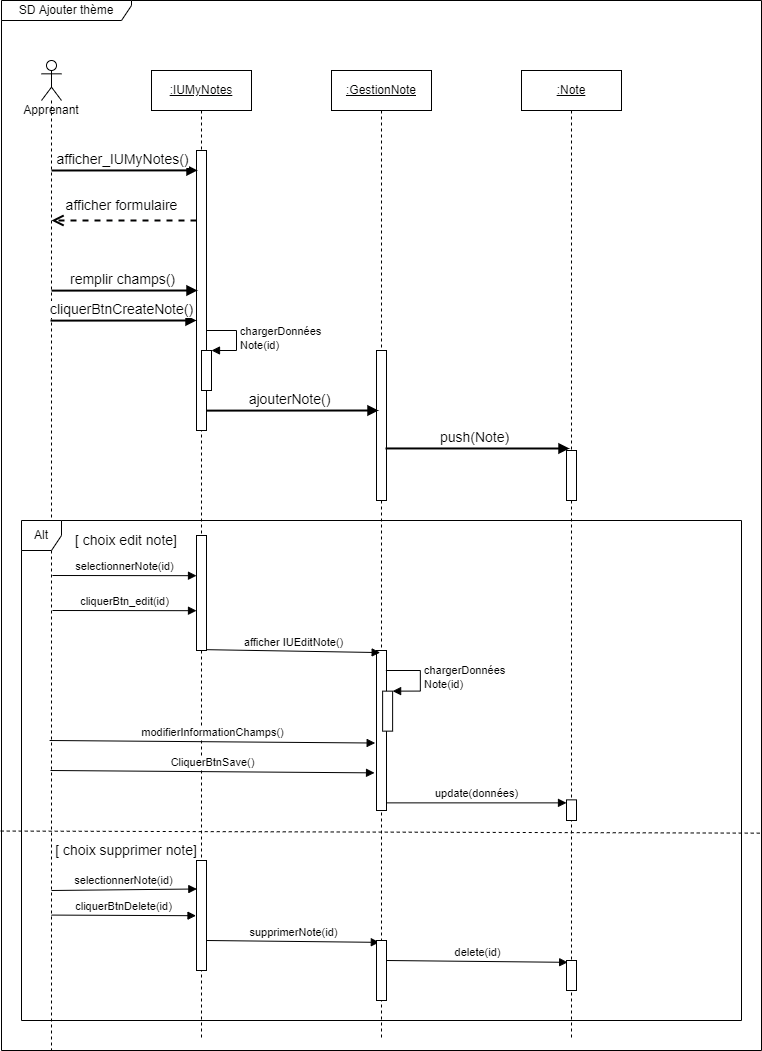
\includegraphics[width=0.75\textwidth]{D) IMAGES/diagseqchap5.png}}
		\caption{diagramme de séquence: Noter Formation}
		\label{Diagramme3}
	\end{figure}
\newpage
\item Diagramme de séquence "S'inscrire"

\begin{figure}[!h]
	\centering
	{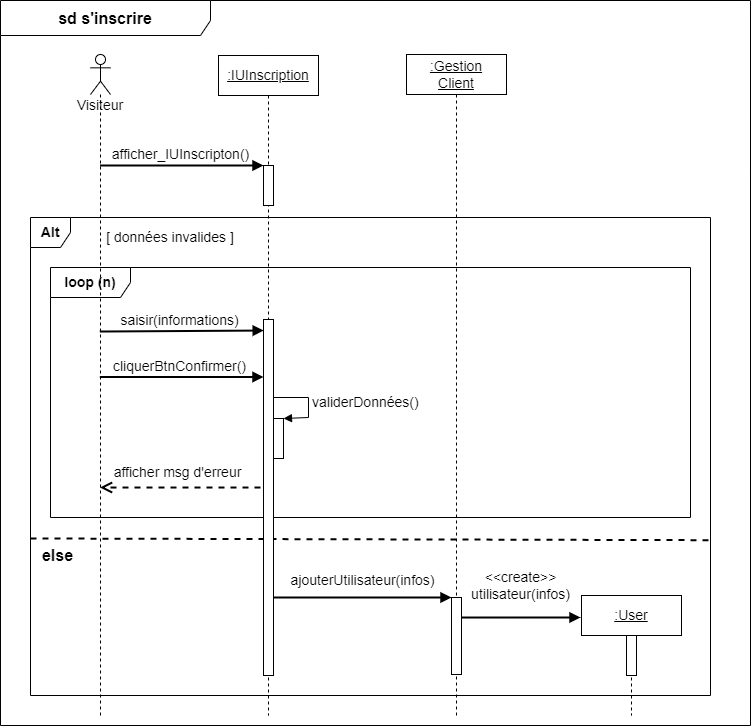
\includegraphics[width=1\textwidth]{D) IMAGES/diaginsc.png}}
	\caption{diagramme de séquence: S'inscrire}
	\label{Diagramme3}
\end{figure}
\end{itemize}
\newpage
\subsection{Diagramme de classes}
La figure ci-dessous correspond au diagramme de classes de notre troisième sprint.

 \begin{figure}[!h]
 	\centering
 	{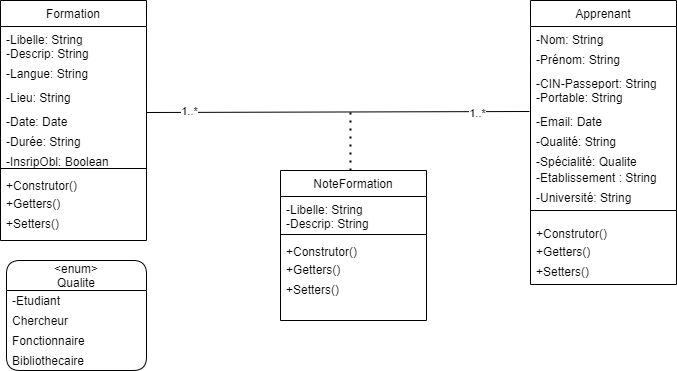
\includegraphics[width=1\textwidth]{D) IMAGES/diagClasse.png}}
 	\caption{Diagramme de classes de sprint 3}
 	\label{Diagramme3}
 \end{figure}
\newpage
\subsection{Diagramme de classe complet}
 \begin{figure}[!h]
	\centering
	{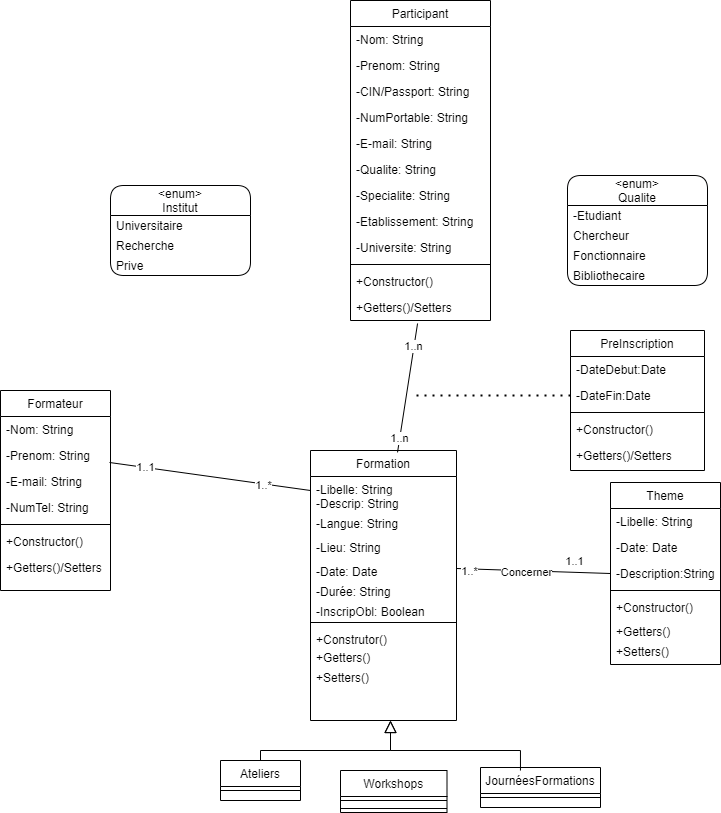
\includegraphics[width=1\textwidth]{D) IMAGES/diagClasseGlobal.png}}
	\caption{Diagramme de classes complet}
	\label{Diagramme3}
\end{figure}
\newpage
\section{Réalisation}
\subsection{Description des interfaces}
\begin{itemize}
	\item Interface: s'authentifier:
		\begin{figure}[!h]
		\centering
		{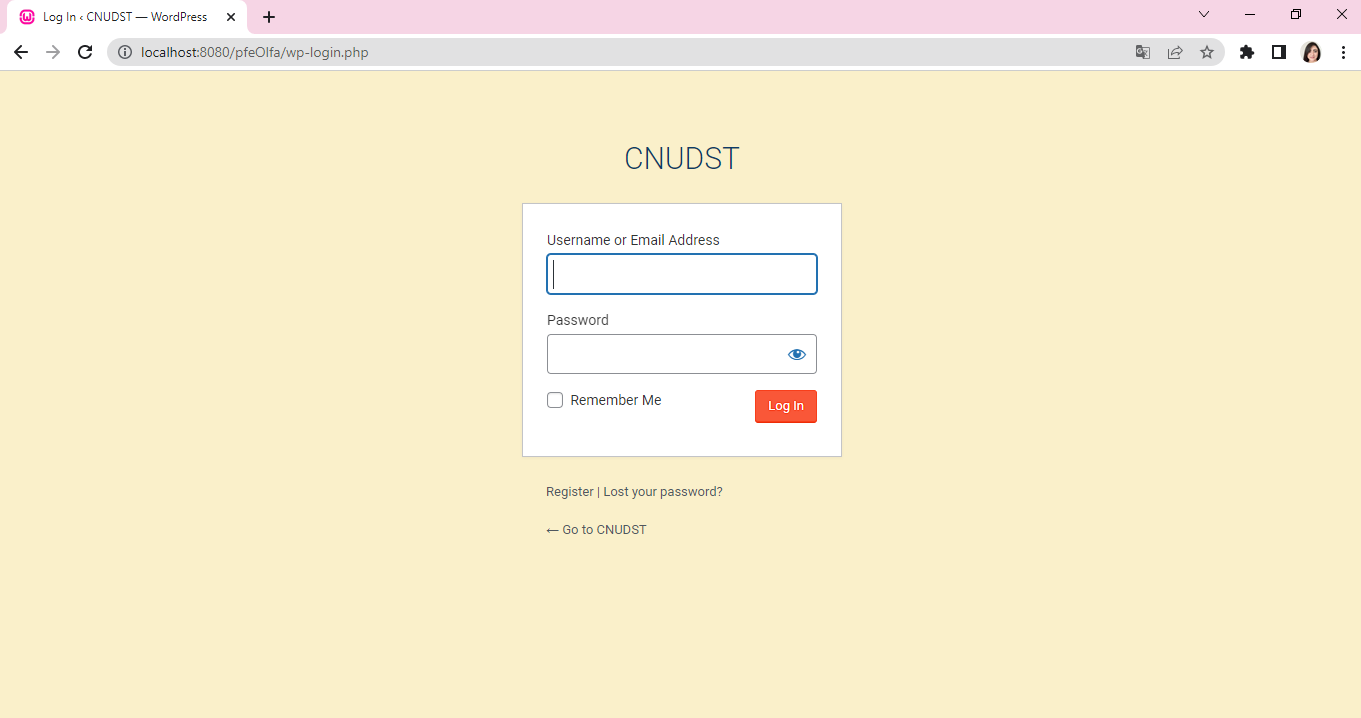
\includegraphics[width=0.95\textwidth]{D) IMAGES/interfauth.png}}
		\caption{Interface: s'authentifier }
		\label{Org}
	\end{figure}

Cette interface permet à un apprenant ou à un administrateur de se connecter, une fois connecté un apprenant a le droit d'ajouter, modifier ou supprimer une note concernant une formation. 
Un administrateur doit s'authentifier pour qu'il puisse gérer le site de CNUDST.
\item Noter Formation
\begin{figure}[!h]
	\centering
	{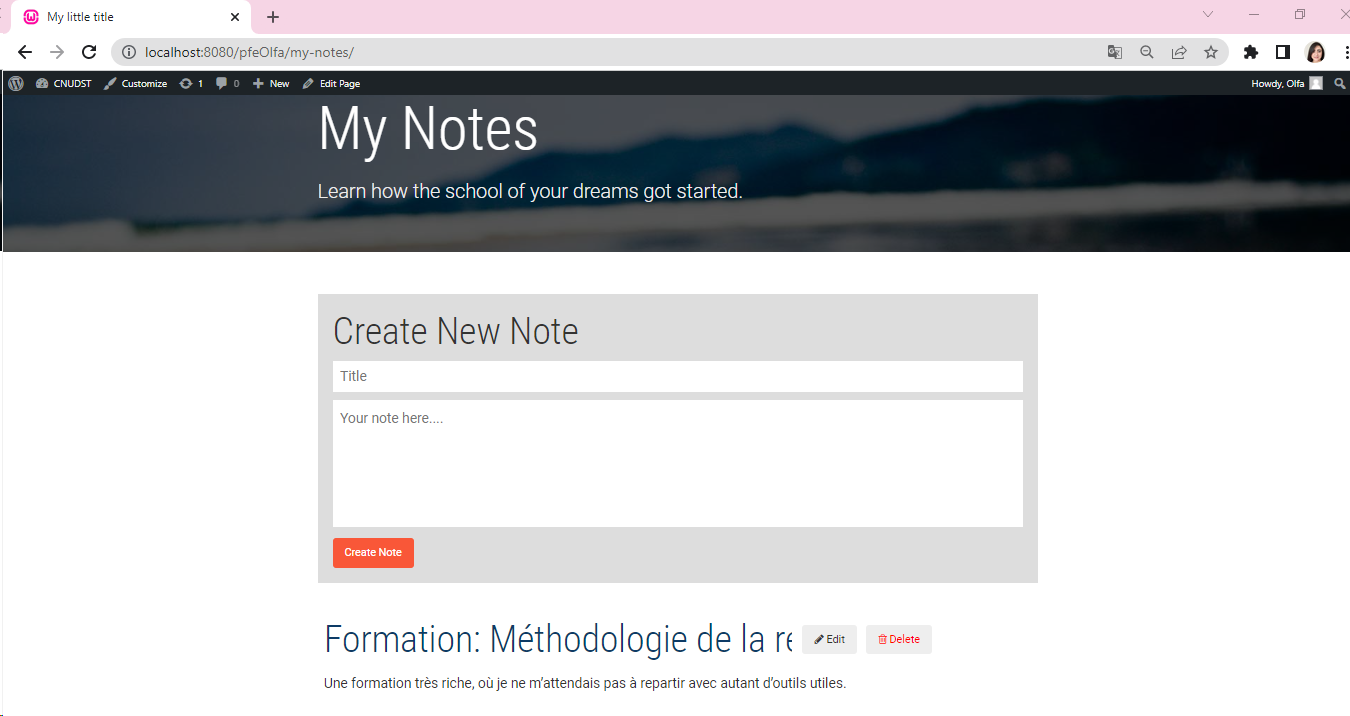
\includegraphics[width=0.95\textwidth]{D) IMAGES/NoteForm.png}}
	\caption{Interface: My Notes}
	\label{Org}
\end{figure}
\\
  Cette interface permet à un apprenant d'ajouter, modifier ou bien supprimer une note concernant une formation.
  \newpage
\item Interface: Détails Formation
  
\begin{figure}[!h]
	\centering
	{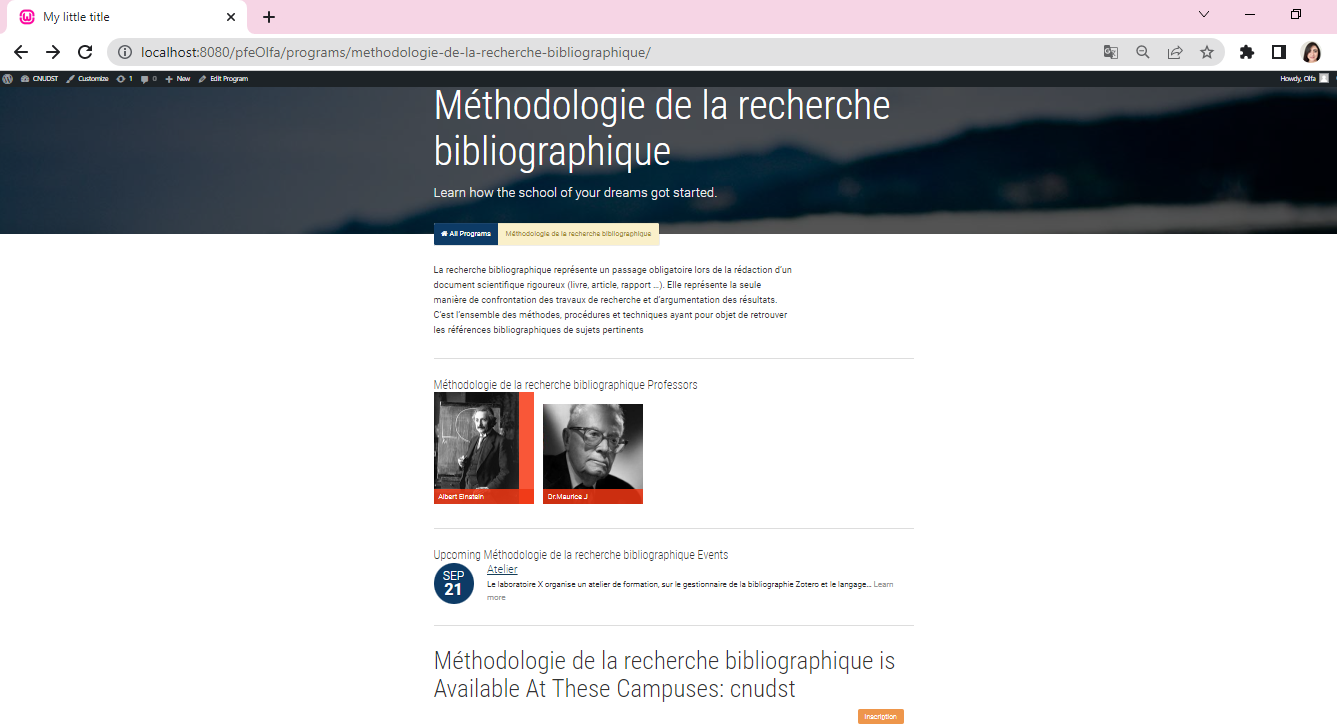
\includegraphics[width=0.95\textwidth]{D) IMAGES/detailform.png}}
	\caption{Interface:Détails Formation}
	\label{Org}
\end{figure}
Au niveau de cette interface il existe le bouton "Inscription" qui permet à un visiteur de s'inscrire à une formation.
\newpage
\item Interface: Formulaire d'inscription.

Un visiteur peut s'inscrire à une formation organisée par le CNUDST via ce formulaire d'inscription. 

 
\begin{figure}[!h]
	\centering
	{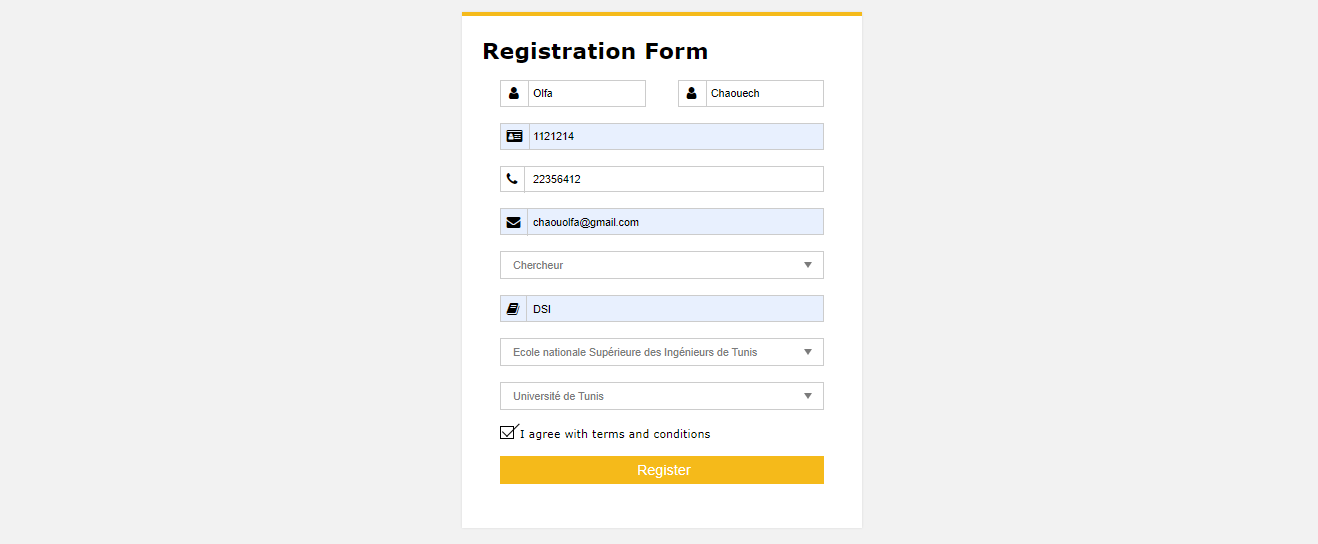
\includegraphics[width= 1\textwidth]{D) IMAGES/Form.png}}
	\caption{Interface:Formulaire d'inscription}
	\label{Org}
\end{figure}

\begin{figure}[!h]
	\centering
	{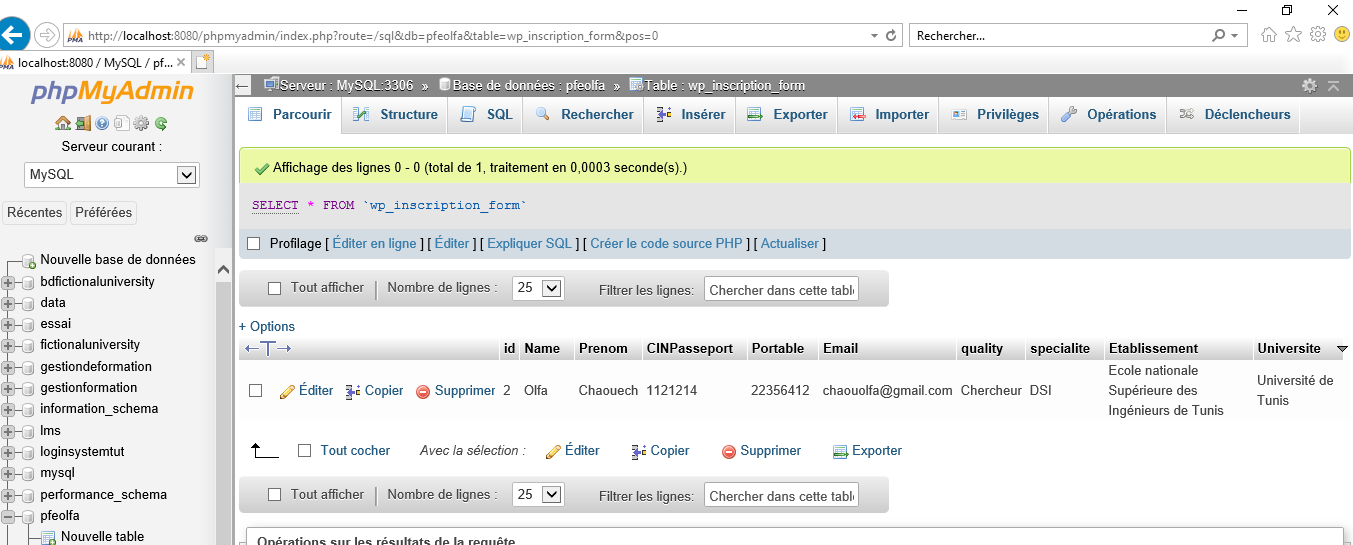
\includegraphics[width= 1\textwidth]{D) IMAGES/db.png}}
	\caption{Insertion effectuée au niveau de la base}
	\label{Org}
\end{figure}
\newpage
\begin{figure}[!h]
	\centering
	{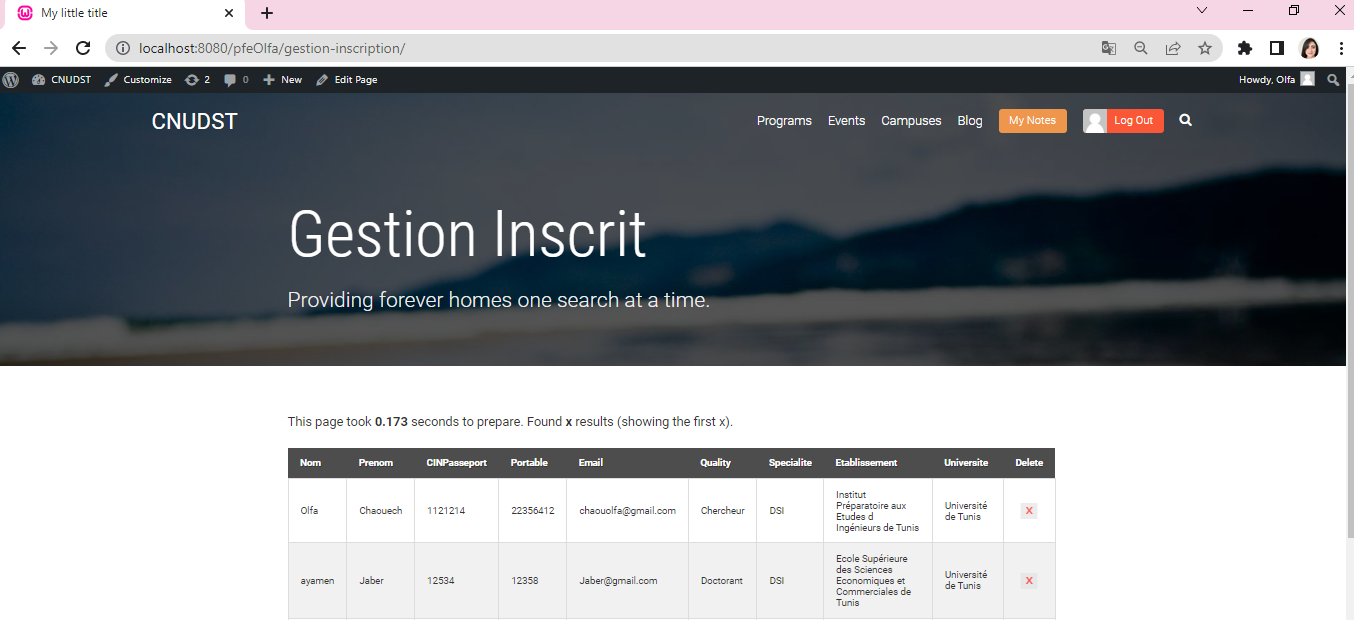
\includegraphics[width= 1\textwidth]{D) IMAGES/GestionInscrit.png}}
	\caption{Gestion Inscription}
	\label{Org}
\end{figure}
Cette interface permet à l'administrateur de consulter et de gérer la liste des visiteurs inscrits
\end{itemize} 
\textbf{Conclusion}\\
Au cours de ce dernier chapitre, nous avons développé notre dernier sprint qui représente la réalisation des six dernières user stories qui composent les EPIC "Inscription à une formation en ligne" et "Interaction sur le site".